\documentclass[11pt, a4paper]{article}
\usepackage{graphicx}
\usepackage{amsmath, bm}
\usepackage{natbib}
\usepackage[utf8]{inputenc}    
\usepackage{natbib}
\usepackage[usenames,dvipsnames]{xcolor}
\usepackage[left=2cm,right=2cm,top=2cm,bottom=2cm]{geometry}
\usepackage{hyperref}
\usepackage[outdir=./]{epstopdf}
\usepackage{lscape}
\usepackage{float}  % PUT FIGURE HERE
\usepackage{multirow}
\usepackage{booktabs} % Create TABS
% \usepackage{array,arydshln}  % CREATE DASH LINE
\title{Identification of stably expressed genes from Arabidopsis RNA-Seq data}
\date{} % Today's date or a custom date



\hypersetup{
    colorlinks,
    citecolor=blue,
    filecolor=blue,
    linkcolor=blue,
    urlcolor=blue
}

\begin{document}
\maketitle

\section*{Abstract}
We examined RNA-Seq data on 165 biological samples from 18 different
experiments carried out by different labs and identified genes that are stably
expressed across biological samples, experiment conditions, and labs. We fit a
random-effect model to the read counts for each gene and decompose the total
variance to into between-sample, between-treatment and between-lab variance
components. Identifying stably expressed genes is useful for count
normalization. The variance component analysis is a first step towards
understanding the sources and nature of the RNA-Seq count variation.


\section{Introduction}

\textbf{Why is normalization important}
RNA sequencing (RNA-Seq) has become the technology of choice for transcriptome
profiling over the last few years. A key task of RNA-Seq analysis is to detect
differentially expressed (DE) genes under various experimental or
environmental conditions. Count normalization are needed for adjusting
differences in sequencing depths or library sizes (total numbers of mapped
reads for each biological sample) due to chance variation in sample
preparation.  In DE analysis, gene expression levels are often estimated from
relative read frequencies. For this reason, normalization is also needed to
account for the apparent reduction or increase in relative read frequencies of
non-differentially expressing genes simply to accommodate the increased or
decreased relative read frequencies of truly differentially expressing genes.

\textbf{Why is stably expressed gene important}
A central idea to many existing count normalization methods is to identify and
use as reference a set of stably expressed genes whose expression levels are
known or expected to not vary much under different experimental conditions.
For example, the trimmed mean of M-values normalization method	(TMM) \citep{robinson2010scaling} and DESeq normalization \citep{anders2010differential}  assume that the majority of
the genes are not DE within an experiment. 
Effectively, these methods use genes with relatively small observed fold
changes under a single experiment as a reference gene set in normalization.
There are two obvious issues with this strategy: 1. The available sample size
in any single experiment may be too small for us to reliably estimate true
fold changes. 2.  If the experiment condition can affect expression levels of
more than half of the genes (\cite{loven2012revisiting}, \cite{wu2013use}),
many of the existing normalization methods (???) may be unreliable. 

\textbf{How to find stably expressed genes}
In pre-genomic era, the so-called "housekeeping genes" (HKGs) are
often considered as candidates of reference genes for normalization (\cite{bustin2002quantification}, \cite{andersen2004normalization}). HKGs are
typically constitutive genes that maintain basic cellular function, and
therefore are expected to express at relatively constant levels in
non-pathological situations.  However, many studies have shown that HKGs are
not necessarily stably expressed (a review can be found in
\cite{huggett2005real} and reference therein).  For example, in the microarray
analysis of the model plant \textit{Arabidopsis thaliana} (Arabidopsis),
\cite{czechowski2005genome} showed that traditional HKGs such as ACT2, TUB6,
EF-1$\alpha$ are not stably expressed, and thus not good reference genes for
normalization.  A similar idea is to use spike-in genes, but
\cite{risso2014nat} showed that spike-in genes are not necessarily stably
expressed and thus may not help normalization.  HKGs or spike-in genes thus
cannot be taken as granted as stably expressed genes for count normalization
purpose.
 
% and careful evaluation should be performed when they are being used in
% normalization. (??? simplify, make concise)

\textbf{Numerically finding stably expressed genes.}
% Why would we bother to study them under RNA-Seq since there are related works in microarray} (some sentense are needed to connect the two paragraphs)
For microarray data, an alternative approach is to numerically find stably
expressed genes by quantifying the variation of measured expression levels
across a large number of microarray data sets. 
For example,  \cite{czechowski2005genome}
measured the expression stability of each gene using the coefficient of
variation (CV). Genes with lower CVs are considered as more stably expressed.
By investigating 721 arrays under 323 conditions throughout development,
\cite{czechowski2005genome} suggested stably expressed (reference) genes under
different experimental conditions for Arabidopsis.
\cite{stamova2009identification} used a different algorithm, geNORM
\citep{vandesompele2002accurate}, to find stably expressed genes based on 526
human blood samples. 
%and  validated a subset of most stably expressed genes they identified.
%Similar studies were carried out for Arabidopsis seed
 \citet{dekkers2012identification}, \citet{gur2009identification}, and
 \citet{frericks2008toolbox} screened a large number of microarray data sets
 to identify stably expressed genes in Arabidopsis seed, breast tumor tissues,
 and mice respectively.
% Similar studies were carried out for Arabidopsis seed
% \citep{dekkers2012identification}, breast tumor
% tissues\citep{gur2009identification}, mouse (universal)
% \citep{frericks2008toolbox} and so on.  
Validation experiments (\cite{czechowski2005genome},
\cite{dekkers2012identification}, \cite{huggett2005real},
\cite{stamova2009identification}) showed that these genes are more stably
expressed than traditional HKGs.  

% Typically, large sets of microarray data are compiled for a given experimental
% condition, and stably expressed genes are validated and recommended for
% potential use. 


\textbf{What is our goal and the approach} 
% RNA-Seq is superior to microarray technology because
% of its high-throughput, pricise measurement, as well as sensitivity for gene
% expressed at both low and very high levels \citep{wang2009rna}. 
In this paper, we discuss numerically identifying stably expressed genes from a large
number of RNA-Seq data sets.
The exponential growth in RNA-Seq study accumulates a large amount of
Arabidopsis data under a variety of experimental/enviromental conditions. We
use generalized linear mixed model (GLMM) \citep{mccullagh1989generalized} to
identify stably expressed genes for Arabidopsis RNA-Seq data. 
We also applied two widely used methods "geNORM"
\citep{vandesompele2002accurate} and  "NormFinder"
\citep{andersen2004normalization} on log-transformed RNA-Seq count data.
We found that the rankings of stably expressed genes provided by the different
methods are consistent (rank correlation $> 0.97$).  Using GLMM will also
allow us to quantify the sources of variation of gene expression. For each
gene, we use three random effect terms to quantify \textit{between-sample},
\textit{between-treatment} and \textit{between-lab} variation. 

\cite{andersen2004normalization} used a linear mixed model to estimate
expression variation in microarray experiments. The variation of
log-transformed expression value is decomposed into intra-group and
inter-group variation for each gene. The stability of that gene in future
experiment is determined by the posterior distribution of error terms after a
Bayesian argument. Genes in a given data set are then ranked by the averaged
stability values, which are defined by absolute value of posterior mean plus
one standard deviation.  RNA-Seq are non-normal count data, in this paper, we
thus choose to use GLMMs to estimate variance components.

(???) Furthermore, new biological insights (REFs) \dots Stably expressed genes
are likely to be involved in basal metabolic or ‘housekeeping’ functions, such
as  kinase activity, nucleotide binding and protein modification processes.
\cite{sekhon2011genome} and \cite{wang2010dynamic} showed that stably
expressed genes are involved in biological processes included cellular
processes, transport, protein modification, translation and signal
transduction by Gene Ontology enrichment analysis. Besides, in expression
study, a high correlation between translational signiture and mRNA level is
found in human stably expressed genes\citep{line2013translational}. In that
paper, an significant increase in mRNA variation prediction was obtained by
selecting genes that are stably expressed in more than 1 tissue.\\

(Limitation and scope) \cite{hruz2011refgenes} pointed out that universally
stably expressed genes may not exist and that a subset of stably expressed
genes from a specific biological context has less variability than those
identified across varying tissues and conditions. Many studies have shown that
genes with stable expression levels  in one experiment are subject to change,
either under varying experimental protocols, or different organs of a given
species (\cite{reid2006optimized}, \cite{hong2010identification}).  It is not
surprising that top 100 stably expressed genes in \cite{czechowski2005genome} shared only 3 genes with top 50  specifically for Arabidopsis seed identified by \cite{dekkers2012identification}.
In this paper, we will analyze gene expression stability both across tissue types
and within tissue types.

% For this reason, we expect that stably expressed genes identified by GLMM  are
% more robust and show less sensitivity toward varying treatments (???).

{\bf Further discussion} Previous studies showed that normalization are needed
to account for nuisance effects, including \textit{between-sample} effects,
e.g., sequencing depths, flow-cell/library preparation effects
(\cite{bullard2010evaluation}, \cite{robinson2010scaling}), as well as
\textit{gene-specific} effects, e.g.,  gene length or GC-contents
(\cite{risso2011gc}, \cite{hansen2012removing}). A number of normalization
approaches are proposed to address different types of unwanted nuisance
effects (\cite{dillies2013comprehensive}, \cite{risso2014nat}). Different from
global-scaling normalization, \cite{risso2014nat}  proposed a regression-based
normalization-remove unwanted variation (RUV).  In that paper, they regressed
the read counts on the known covariates of interest (e.g. treatment effects)
and unknown factors of nuisance effects. The factors of nuisance effects are
estimated from a subset of data, and are then adjusted for in DE analysis. In
RUVg approach, they are estimated through a factor analysis. A main assumption
for RUVg is that a set of stably expressed genes can be identified first
.

\section{Data}
 We obtained 165 biological samples of Arabidopsis  from 18 experiments from \textit{Gene Expression Omnibus} (GEO) at \textit{National Center for Biotechnology Information}  ( NCBI, \url{http://www.ncbi.nlm.nih.gov/}).  A brief description of the experiments can be found in supplementary material. More details for each experiment are also accessible at NCBI via the unique accession number provided.
 
\textbf{From FASTQ to Read Count} Read counts were obtained by processing
zipped FASTQ data in three steps. First, Sequence Read Archive (SRA) format
files of Arabidopsis samples were retrieved from GEO, and then converted to
FASTQ files using \verb"SRA Toolkit"(version 2.3.5-2). Next, the reference
genome of Arabidopsis was downloaded  through the Ensembl plants FTP server
(\url{http://plants.ensembl.org/info/data/ftp/index. html}). As suggested by
\cite{anders2013count},  "FASTA(DNA)" link rather than "FASTA(cDNA)" was
selected because samples were aligned to the genome, not the transcriptome.
The index  was built subsequently for reference genome.  Lastly, Short reads
in FASTQ were  aligned to reference genome by  \verb"align()" and read counts
were summarized by \verb"featureCounts()" in R package \verb"Rsubread"
(version 1.14.2,  \cite{liao2013subread}). We used default options except that
the annotation file is set to be \verb"Arabidopsis_thaliana.TAIR10.22.gtf".
The multi-mapping or multi-overlapping reads were not counted.  


\textbf{Consider there subsets} 
We first want to identify stably-expressed genes among ** seedling samples
from ** labs.



The 18 labs were grouped and managed into three data sets by tissue type.
\cite{czechowski2005genome}, \cite{hruz2011refgenes}, and
\cite{dekkers2012identification} showed that transcriptomes vary across
different tissue types or development stages. For this reason, we prepared
three read counts matrices, formed in the way that rows denote gene and
columns indexes biological sample. \textbf{Set 1} consists of 72 biological
samples that came from 9 labs of Arabidopsis seedling (aged 2 days to 10 days)
experiment under 29 treatments (different in terms of environmental conditions
or genotypes, same thereafter); \textbf{Set 2} has a sample size of 39 from 5
distinct tissue type experiments (flower, leaf, seed, carpel and hypocolty)
with 16 treatments; \textbf{Set 3} consists of 5 lab experiments conducted
specifically for leaf, with a total number of 60 biological samples among 28
different treatments. Note that  Set 2 and Set 3 overlap with each other by
lab experiment GSE48235 (6 samples). Samples within each group were merged by
their unique gene IDs, and then stored in the read count matrices.  \\




\section{Methods}
\subsection{Remove lowly-expressed genes} Prior to normalization, we removed non-informative rows, such as features that were not of interest or those that had low overall counts, as suggested by \cite{anders2013count}. Filtering non-informative genes is helpful not only because rows with small read counts provides little information about expression level,  but also that such rows will cause convergence failure in the regression models. In practice,  we found selecting genes by a mean count of at least 3 would effectively avoid computational issue.  By removing genes with less than 3 reads per sample, we obtained a matrix of 22334 genes by 72 samples for set 1, 25239 by 39 for set 2, and 21290 by 60  for set 3.  

\begin{table}[h]
\centering
\begin{tabular}{lrrrr} \hline
& \# of labs & \# of treatments  & \# of biological samples & \# of genes \\ \hline
Set 1 &9 & 29 &72  &22334  \\
Set 2 &5 & 16 & 39 &25239  \\
Set 3 &5 &28  &60  & 21290\\ \hline
\end{tabular}
\end{table}

%\textbf{Moved from introduction part, or better to put it in discussion part?}
%\cite{czechowski2005genome} and \cite{dekkers2012identification} adopted similar approach for statistical analysis for identifying stably expressed genes, and both used Arabidopsis microarray data. Briefly, for each gene the mean expression and the standard deviation (SD) over all biological samples are calculated, and the coefficients of variation (CV), which is the ratio of SD to mean expression, are obtained. Genes with lower CVs are expected to be more stably expressed. This simple approach, however, does not provide us any information about possible sources, except the amounts,  of variation.  \textbf{Since it is often observed that genes with higher expression levels tend to have smaller dispersion, this simple approach will inevitably choose those genes. [Hruz 2011] Selection Bias}\\ 

\subsection{Count Normalization}
Briefly, a pseudo-reference sample is created by taking the geometric mean across samples for each gene. Then the normalization factor for sample $j$ is estimated as the median of the fold-changes between sample $j$ and reference sample over all genes.

The term $\log(R_{jkl}N_{jkl})$ serves as an offset, where  $ R_{jkl}$ is library size and  $N_{jkl}$ is the normalization factor calculated by DESeq normalization \citep{anders2010differential}. 

\subsection{Poisson log-linear mixed-effects regression model} 
% (Each individual count is model as a Poisson distribution. The count mean is
% modeled through a log-linear mixed-effects regression model.)

Let $Y_{ijkl}$ denote the read count for $i$th gene
in $j$th observational unit of $k$th treatment group in $l$th experiment (lab)
and index $i$ is suppressed herein since only one gene is evaluated at a time
by regression model. We assume that each read count follow a Poisson
distribution,  
\[Y_{jkl}\sim \text{Poisson}(\mu_{jkl}).\] 
We use a log-linear Poisson regression model to capture 
the variation of $\mu_{jkl}$ across samples and experimental conditions (treatments,
organs, etc.),
\begin{equation}\label{q1}
    \log( \mu_{jkl}) = \xi + \log(R_{jkl}N_{jkl})+ \alpha_l + \beta_{k(l)} + \epsilon_{jkl} 
\end{equation}
where $\alpha$'s are the effects for labs,  $\beta$'s are treatment effects
nested in labs, and $\epsilon$'s are the effects for biological samples. 
The term $\log(R_{jkl}N_{jkl})$ are the normalization factors discussed in
subsection (REF).

[Why treat lab-effect as random-effect] We view the collected data sets as a random sample from the pool of all
Arabidopsis RNA-Seq experiments. \dots generalized inference \dots
For the same reason, we also consider the treatment effects as random effects
in the sense the treatment effect will be different in future experiments.

It is assumed that $\alpha$'s, $\beta$'s and $\epsilon$'s are mutually
independent, and  
%   \[ \log( \mu_{ijk}) = \xi + \log(R_{ijk}N_{ijk})+ \alpha_k + \beta_{j(k)} + \epsilon_{ijk} \]
  \[\alpha_l\sim N(0, \sigma^2_1),\] 
  \[\beta_{k(l)}\sim N(0, \sigma^2_2),\]
   \[\epsilon_{jkl}\sim N(0, \sigma_0^2).\]
$\sigma_0^2$, $\sigma_1^2$, $\sigma_1^2$ are called variance-components. They capture the
between-sample, between-treatment variation and between-lab variation
correspondingly.
[We need to be clear about which component capture what kind of
variation, ecotype? treatment? growing conditions? age?] 
The between-sample variation capture extra-Poisson variation in read counts
within a treatment group. It plays a similar role as the dispersion parameter
in a negative binomial model (REFs).



\subsection*{ Estimation of
Variance Components
and
Identification of Stably Expressed Genes 
}

We estimate the variance components from (\ref{q1}) for each gene using
likelihood-based methods (details provided below).  The
genes are then ranked  in ascending order by their magnitude of total
variation, quantified by $\sigma^2 = \sigma^2_0 + \sigma_1^2 + \sigma_2^2$.
Top ranked genes are considered to be most stable in terms of expression
value. 


The joint density function of $\bm Y=(Y_{jkl})'$ given $\bm \mu= (\mu_{jkl})'$ is 
  \[f(\bm Y|\bm \mu )=\prod_{ j, k,l}f(y_{jkl}|\mu_{jkl})=\prod_{j,k,l}\frac{[\mu_{jkl}]^{y_{jkl}}\exp(-\mu_{jkl})}{y_{jkl}!}\]
A re-expression of  (\ref{q1}) in matrix form gives 
\[\log\bm \mu= \bm \xi + \log{\bm{NR}} + \bm {Z_1\alpha} + \bm{Z_2\beta} + \bm \epsilon \]
where $\bm \xi = \bm 1\cdot\xi$ and $\bm 1$ is a vector of 1s, $\bm Z_1$ is the design matrix for random effect $\bm \alpha=(\alpha_l)$, and $\bm Z_2$ is the design matrix for random effect $\bm \beta $. 
Therefore  $\bm\mu  \sim \log N(\bm \mu_0, \bm \Sigma)$ where 
$$\bm \mu_0 =\bm\xi + \log(\bm {NR}),$$ 
$$\bm \Sigma = \sigma_1^2\bm {Z_1Z_1'} + \sigma_2^2\bm {Z_2 Z_2'} +\sigma_0^2 \bm I$$
and $\bm I$ is of dimension $Q$ where $Q$ is the total number of biological samples. 
 And 
 \[f(\bm \mu |\bm \mu_0, \bm \Sigma)=\prod_{j,k,l} \mu_{jkl}^{-1}\cdot \frac{1}{ \sqrt{(2\pi)^Q|\bm\Sigma|}}\exp[-\frac{1}{2} {(\log\bm \mu - \bm \mu_0)^T\bm \Sigma^{-1}(\log\bm \mu - \bm \mu_0)}]\]
 the joint density is then
  \[f(\bm Y, \bm \mu |\bm \mu_0, \bm \Sigma) =\frac{1}{\sqrt{(2\pi)^Q|\bm \Sigma|}}\exp[-\bm 1^T\bm \mu - -\frac{1}{2} {(\log\bm \mu - \bm \mu_0)^T\bm \Sigma^{-1}(\log\bm \mu - \bm \mu_0)}]\prod_{jkl}\frac{[\mu_{jkl}]^{y_{jkl}-1}}{y_{jkl}!}\]
   Therefore the likelihood function or the marginal distribution is 
   \begin{equation}\label{q2}
   L(\xi, \sigma_1^2, \sigma_2^2, \sigma_3^2|\bm Y)=f(\bm Y|\bm \xi, \bm \Sigma)= \int_{\bm{\alpha,\beta,\epsilon}} f(\bm Y, \bm \alpha, \bm \beta, \bm \epsilon |\bm \mu_0, \bm \Sigma)d\bm \alpha d \bm\beta d\bm \epsilon 
   \end{equation}
where the integral in (\ref{q2}) can be approximated by Gaussian-Hermite (GH) quadrature. The estimate of $\bm\theta = (\xi, \sigma_0^2, \sigma_1^2, \sigma_2^2)'$ is obtained by maximizing the log-likelihood after GH approximation.  This procedure is done with \verb"glmer()"  in \verb"lme4"  package (\cite{bates2012lme4}, version 1.1.7)  with option  "optimizer= 'bobyqa' " 
 

 %\citep{mcculloch2001generalized}.
 %Model (\ref{q1}) allows us to take into account the design structure for each data set. We assume that genes are mutually independent [Maybe we don't need it here.]. 
  
 \section{Results}
 
 \subsection{Stably Expressed Genes}
 [\textbf{The interesting genes}]
  For each of the three sets, we selected top 100 stably expressed genes (see supplementary material for detail). %The mean read counts of top 100 vary from less than 10 to more than 6,000, constituting a broad range of expression values. This shows that our approach has negligible bias regarding expression level in selecting stably expressed genes. 
Comparison of the three lists reveals that they share four genes in common, that is, "AT1G52630", "AT1G54610", "AT4G26965" and "AT5G47790".  Those genes are stably expressed under different experimental conditions and tissue types, and thus may be worth further study. AT1G13320 was identified  as a stably expressed gene under all six experimental conditions by \cite{hong2010identification} analyzed, and it was also found to be present in 6 of 10 stably expressed gene lists in\cite{czechowski2005genome}.  Here, AT1G13320 is ranked 4, 357, 151 for the three sets we examined, making it a good candidate for reference gene.

[\textbf{How does stably expressed genes compare to each other?}]
Next, we compared the stably expressed genes to reference ones identified under microarry studies and further validated by variants of PCR expression analyses (e.g., qRT-PCR in \cite{czechowski2005genome} and RT-qPCR in \cite{dekkers2012identification}). The normalized count values  (i.e. read counts multiplied by a factor of  $10^6$/library sizes) by \cite{anders2013count} give a \textit{Count per Million} (CPM) interpretation.  We randomly chose 5 stably expressed genes from Set 1 (AT1G30470, AT2G30880, AT3G63150, AT4G26965 and AT5G13300) to compare gene expression level with 5 traditional HKGs  (AT1G13440, AT3G18780, AT4G05320, AT5G12250, AT5G60390) and 5  reference genes  for developmental series (AT1G13320, AT5G59830, AT2G28390, AT4G33380 and AT4G34270, Figure 1 of \cite{czechowski2005genome}). The left panel of  Figure \ref{expressinlevel} shows the CPM of the 15 genes. We confirmed Czechowski's conclusions that traditional reference genes are not necessarily stable ones (top left); also, Czechowski's reference genes are relatively more stable in terms of expression level (middle left); furthermore, an even higher level of expression stability is achieved (bottom left), implying better candidate reference genes for normalization in RNA-Seq study. We used Set 2 to compare expression stability with Dekkers et. al., because we didn't require any specific tissue type in that analysis and  it is expected that stable genes identified in Set 2 would also apply to Arabidopsis seed. The right panel of Figure \ref{expressinlevel} reveals the same pattern as described in Set 1 comparison: seed specific reference genes are much better than "classical" HKGs, yet they may be outperformed by other genes.  The same scenario applies for leaf-specific RNA-Seq data of Set 3 (see supplementary Figure \ref{sup:expressinlevel}).  %Genes with smaller total variance $\sigma^2$ are more stably expressed. 

 \begin{figure}[H]
\begin{center}
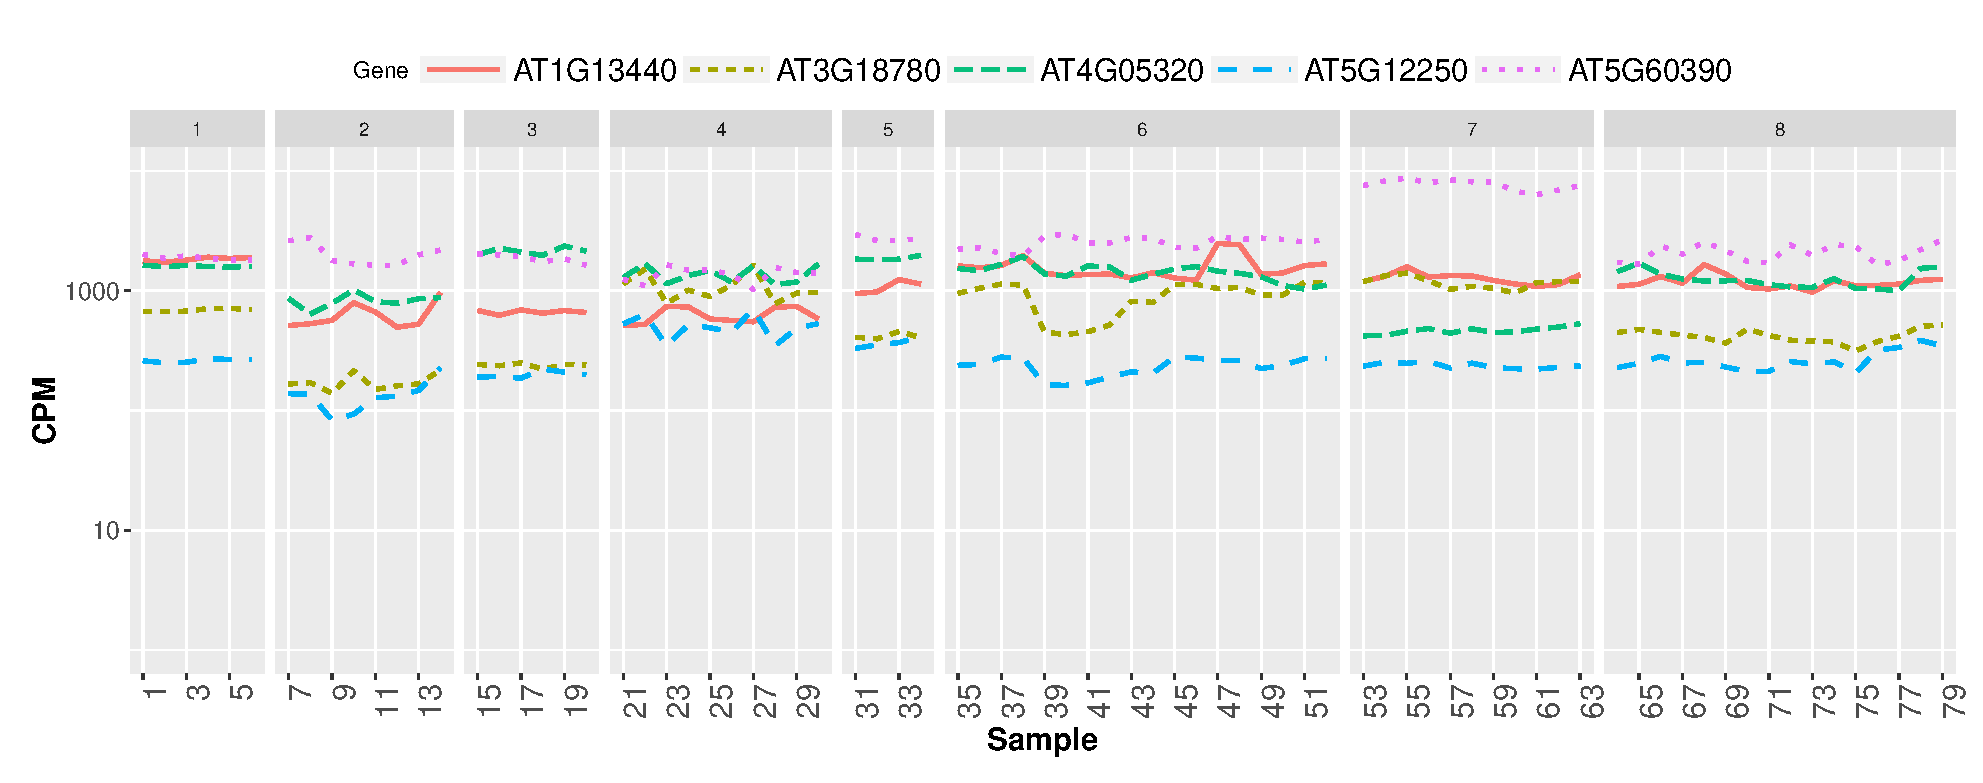
\includegraphics[scale=0.4]{../Figures/A1.eps}
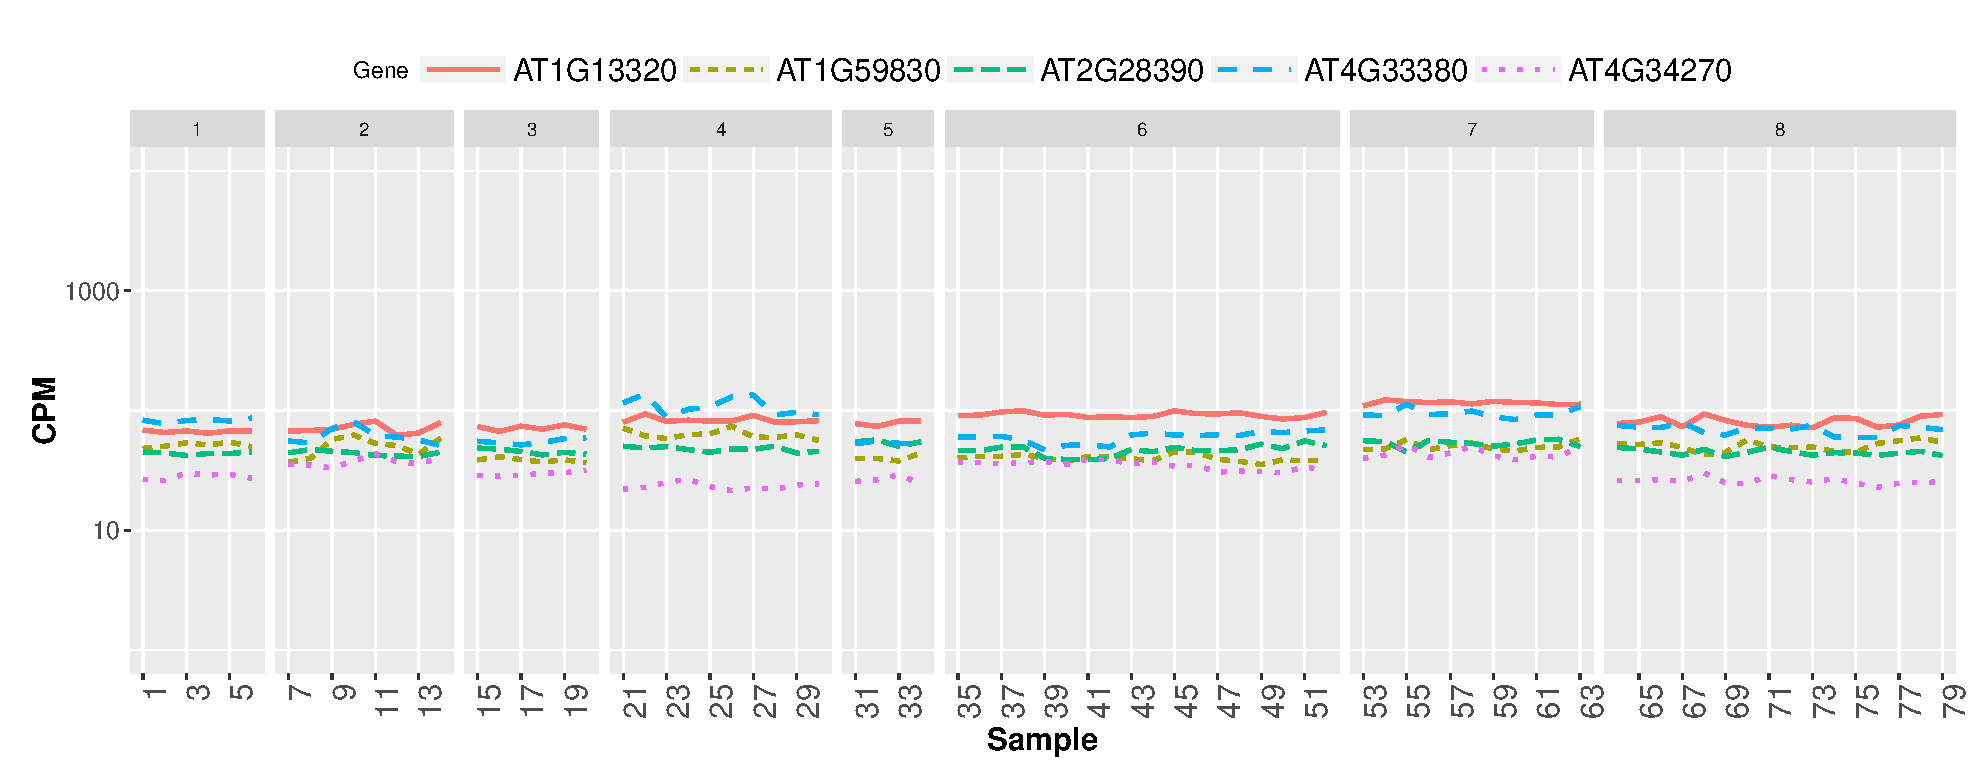
\includegraphics[scale=0.4]{../Figures/A2.eps}
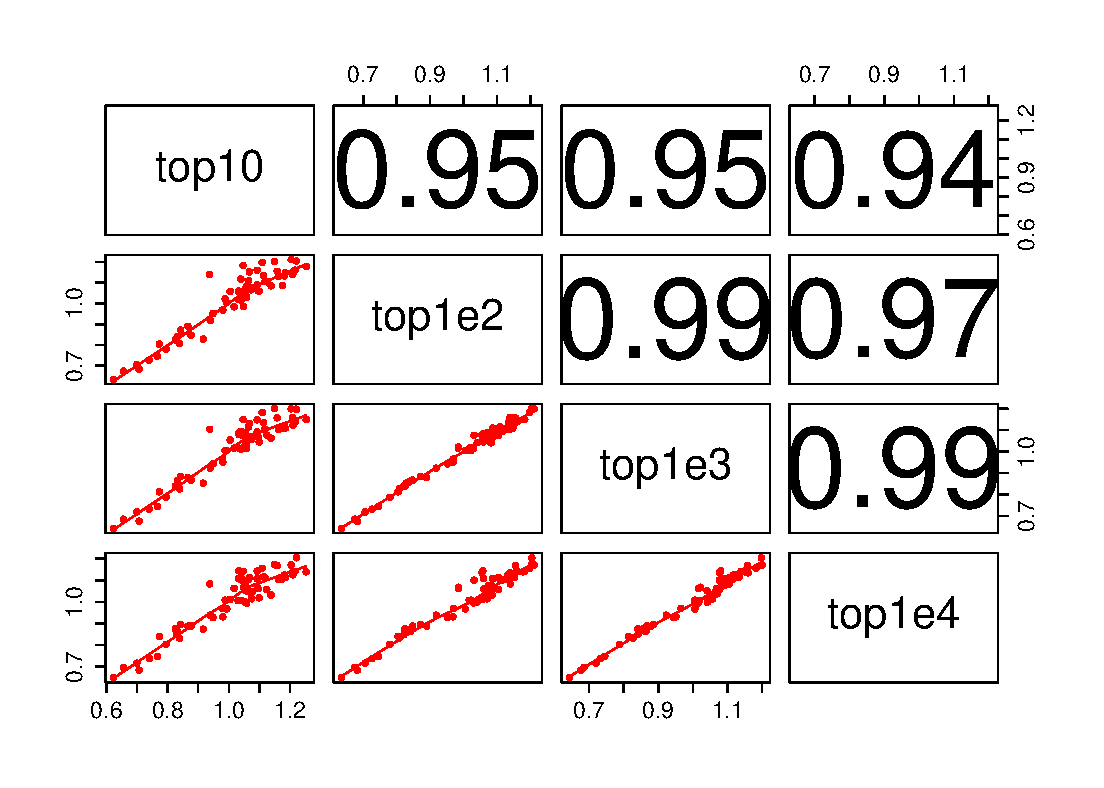
\includegraphics[scale=0.4]{../Figures/B1.eps}
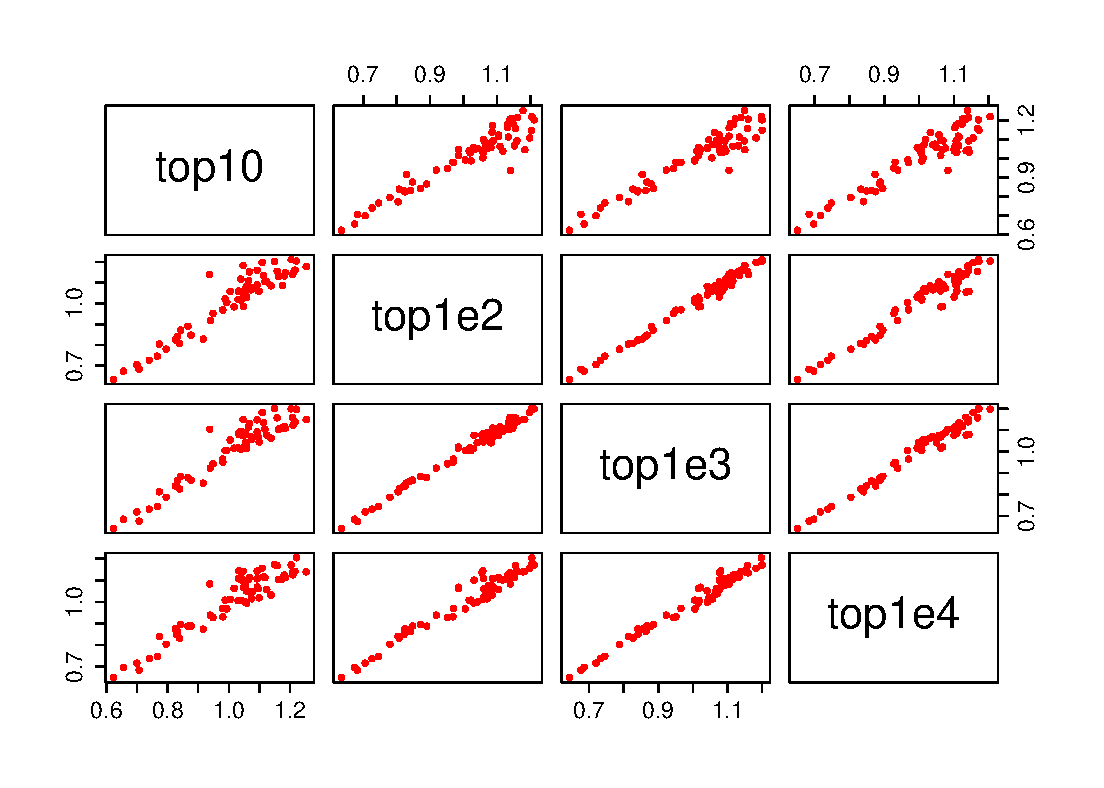
\includegraphics[scale=0.4]{../Figures/B2.eps}
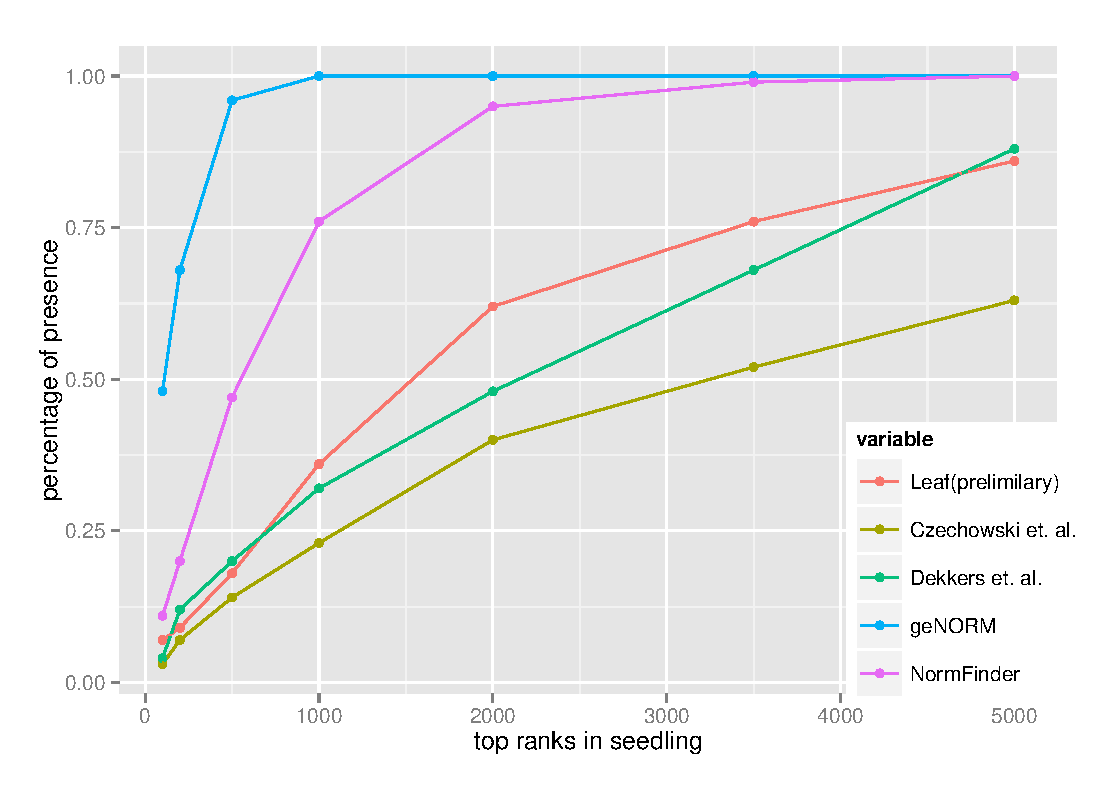
\includegraphics[scale=0.4]{../Figures/C1.eps}
\includegraphics[scale=0.4]{../Figures/C2.eps}

\caption{{\small{\label{expressinlevel} Expression levels  count-per-million (CPM) of genes across RNA-Seq samples. Left panel for seedling data:  5 traditional reference genes (top)};  5 stably expressed genes by Czechowski et. al. (middle) ; 5 stably expressed genes identified by total variance (bottom). Right panel for tissue data: 5 classical HKGs (top);  5 stably expressed genes from Dekkers et. al. (middle) ; 5 stably expressed genes identified by total variance (bottom) }}
\end{center}
\end{figure} 

To further confirm the stability of gene expression, the geNORM \citep{vandesompele2002accurate} procedure and %its R implementation \verb"NormqPCR" \citep{kohl2013package} 
NormFinder \citep{andersen2004normalization} 
 were used to analyze putative reference genes given above.  For each gene, an average expression stability ($M$) is calculated by a pairwise comparison within the reference set across all samples. This procedure is repeated through a stepwise elimination of least stably expressed genes, after which genes are ranked in the way that lower $M$ value genes are more stably expressed \citep{vandesompele2002accurate}. This analysis supports our conclusion that of, the genes considered, the genes we identified are more stable than reference genes by Czechowski et. al., and that traditional HKGs are among the least stable (Figure \ref{mvalue}). Next, when looking at all the genes analyzed, there is high consistency between the ranks of $M$ value and total variance $\sigma^2$: the spearman correlation is 0.99. We also did similar study for Set 2 and Set 3, and the pictures remained the same (see Supplementary Figure \ref{sup:mvalue}). The spearman correlations  between ranks by total variance and by NormFinder are 0.975, 0.97 and 0.945 for the three sets respectively, showing a consistency between the two methods. 

 \begin{figure}[h!]
\begin{center}
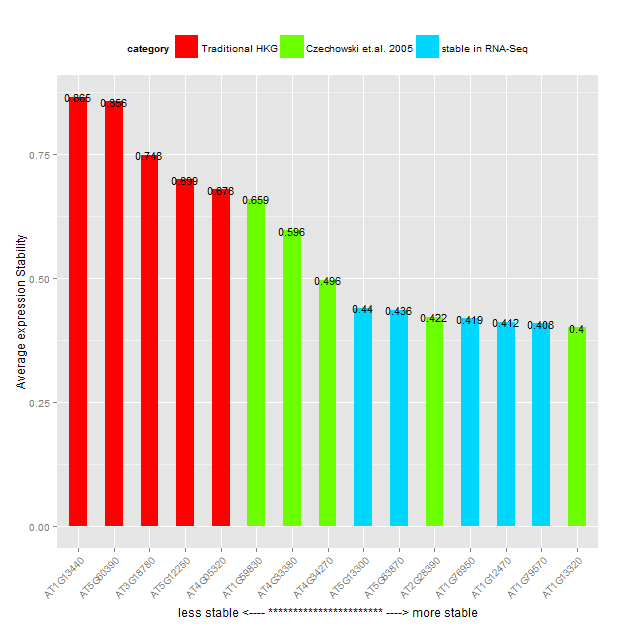
\includegraphics[scale=0.5]{../Figures/mvalue1.png}
\caption{\label{mvalue} geNORM ranking of reference genes: 5 traditional HKGs, 5 reference genes identified by Czechowski et. al. and 8 stably expressed genes based on seedling RNA-Seq data.  More stable genes are indicated by lower average expression stability values M.  }
\end{center}
\end{figure}


It is worth pointing out that a  portion of reference genes suggested by Czechowski et. al. and Dekkers et. al. are good, if not the best,  candidates for normalization. Investigation into Top100 in Czechowski et al. and Top50 in Dekkers et al. reveals certain consistency between sets of stably expressed genes. Of the top 100 genes (developmental series) in  Czechowski, 88 are present in Set 1 we analyzed (89 for Set 2, and 88  Set 3, respectively). Table \ref{table:stablegenerank} summarizes the percentage of presence when we consider top 100, 500, 1000 and 5000 stable genes.  We also observed that the list of reference genes suggested by Dekkers are slightly less consistent (see table \ref{table:stablegenerank} for detail). A hypergeometric distribution was used to test the statistical significance. Let $N$ be the total number of genes considered, $K$ the number of genes in reference list (for Czechowski $K=100$ or for Dekkers $K=50$), $n$ the number of top stably expressed genes we identified,  and $X$, the number of genes confirmed as stably expressed.  If $X$ were totally random, then it follows a hypergeometric distribution $P(X = k) = {K \choose k}{N-K \choose n-k}/{N\choose n}$. It is not practical to calculate the exact $p$ value due to large $N$. The simulated $p$ values by re-sampling  were 0 for all situations. This approach is not accurate due to ignoring the correlation between genes, which may be anti-conservative and lead to false positives. Nonetheless this test is at least informative.  
\begin{table}[ht]
\label{table:stablegenerank}
\begin{tabular}{lrrrr r rrrr} \hline
 & \multicolumn{4}{c}{Czechowski (developmental series)} & & \multicolumn{4}{c}{Dekkers (seed)} \\ \cmidrule(r){2-10}
Top   &   100  & 500     & 1000     & 5000  &  & 100    & 500    & 1000    & 5000    \\ \hline
Set 1 &  5(5.7\%)   & 16(18.2\%)  & 29(33.0\%)  &70(79.5\%)  & &2(4\%)  &  4(8\%)  &10(20\%) & 38(76\%)   \\
Set 2 & 4(4.5\%)    &17(19.1\%)   & 31(34.8\%)  &77(86.5\%) & &2(4\%)  &  4(8\%)  &10(20\%) & 38(76\%)   \\
Set 3 &4(4.6\%)     &17(19.3\%)   &27(30.7\%)   &76(86.4\%) &  &1(2\%) & 9(18\%) &15(30\%)  & 42(84\%) \\ \hline 
\end{tabular}
\caption{Number (percentage) of genes present in the top 100, 500, 1000, 5000 list. }
\end{table}
Next, we explored the consistency between stably expressed genes identified from the three sets in this study. Note that experimental data are from different labs except only 1 lab with a sample size of 6 was overlapped between Set 2 and Set 3. This comparison shows that stably expressed genes are slightly more consistent within RNA-Seq data than between RNA-Seq and microarray data (Figure \ref{fig:rankVSrank_RNA}). % Supplementary figure \ref{fig:rankAgainstrank} present rank-rank plot of Set 1 versus Set 2 and Set 1 versus Set 3.  

 \begin{figure}[h!]
\begin{center}
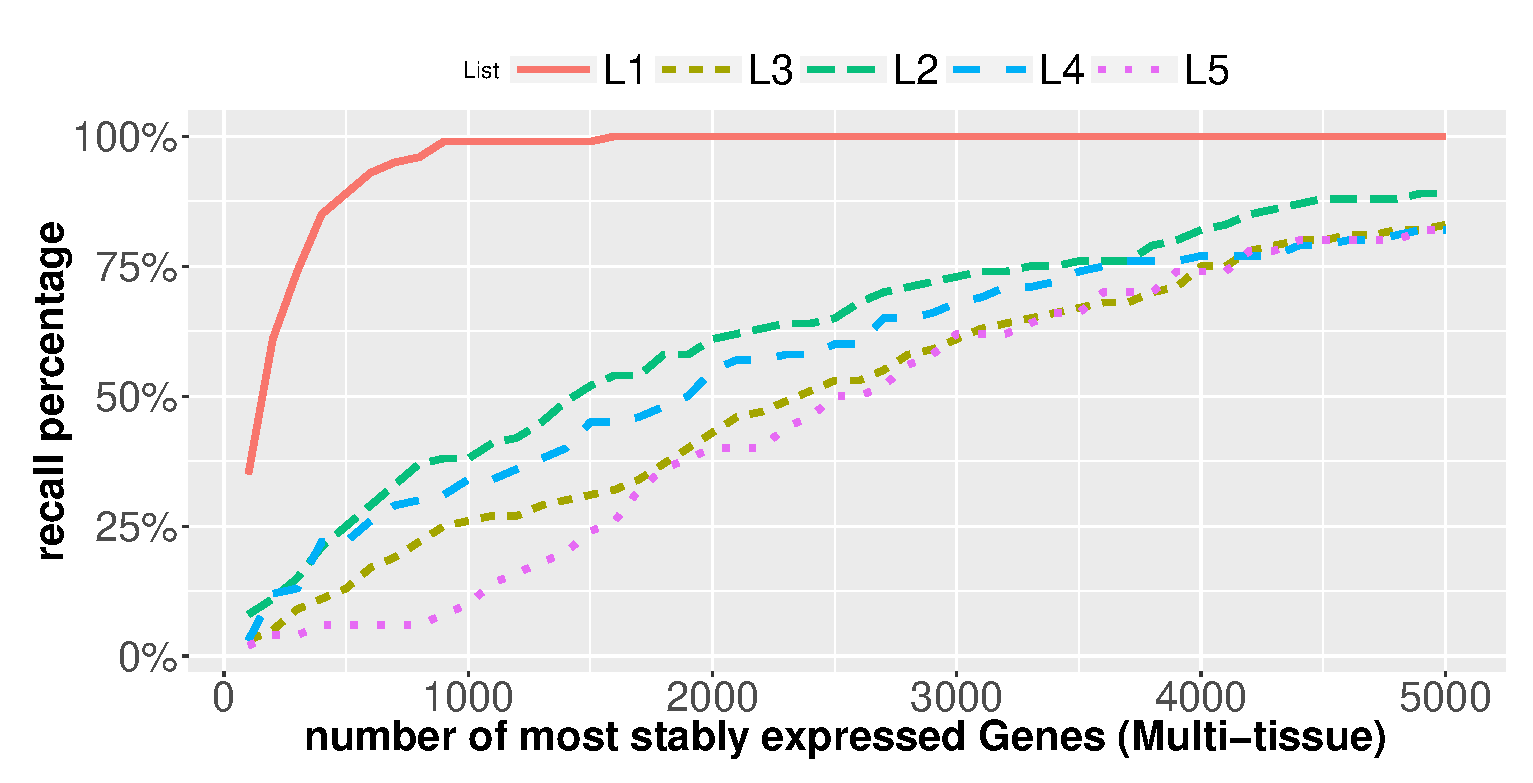
\includegraphics[scale=0.6]{../Figures/rankVSrank_RNA2.eps}
\caption{\label{fig:rankVSrank_RNA} the percentage of genes present in seedling rank list. For example, ''Tissue" means that, of the top 100 stable tissue genes, the percentage of presence in top stable seedling genes.}
\end{center}
\end{figure}



  \subsection{Sources of variation}
 One nice feature about random effect model (\ref{q1}) is that it allows us to decompose total variance into 3 variance components for each gene. With the variance components estimated, we are able to tell how much each component contributes to total variation.  As shown in Figure \ref{densityplot}, between-lab variance component explains the largest part of the total variation (averaged across all genes, 76.7\%, 67.5\% and 52.8\%  for Set 1, Set 2, and Set 3 respectively).  The second largest variation comes from treatment level (16.2\%, 21.4\% and 25.0\%, same as above), whereas biological sample has the least amount of variation(7.1\%, 11.1\% and 22.1\% respectively, same as above).  The plots also reveal that expression levels are less variable within seedling (left) or leaves (right) than across different tissue types (middle panel) since the overall variances are larger when different tissues are considered.  

\begin{center}
\begin{table}[h]
\centering
\begin{tabular}{lrrr} \hline
&lab variation & treatment variation & sample variation  \\  \hline
Seedling  &76.7\% &16.2\% &7.1\%  \\
   Tissue  &67.5\% &21.4\% &11.1\%  \\
     Leaf   &52.8\% &25.0\% &22.1\% \\ \hline
\end{tabular}
\caption{\textbf{Ready to delete}}
\label{table:percentageofvariation}
\end{table}
\end{center} 
 
 \begin{figure}[h]
\begin{center}
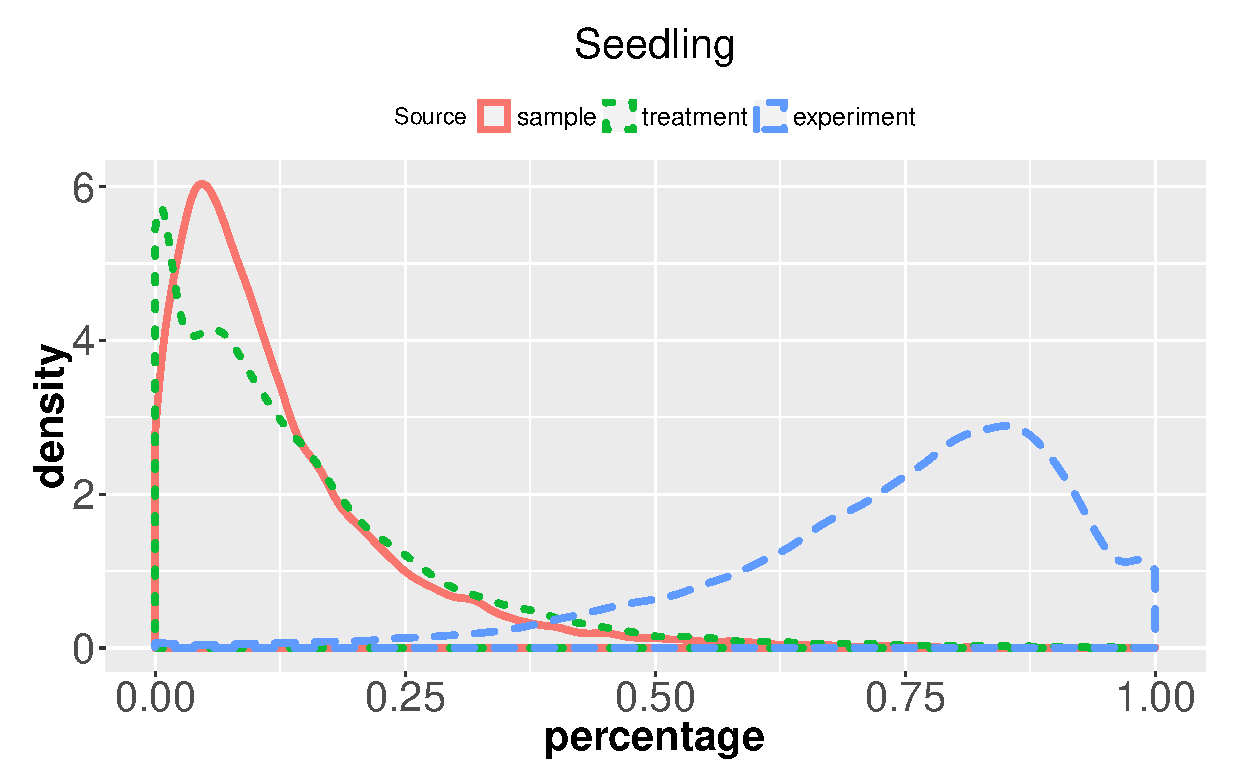
\includegraphics[scale=0.3]{../Figures/var_dens1.eps}
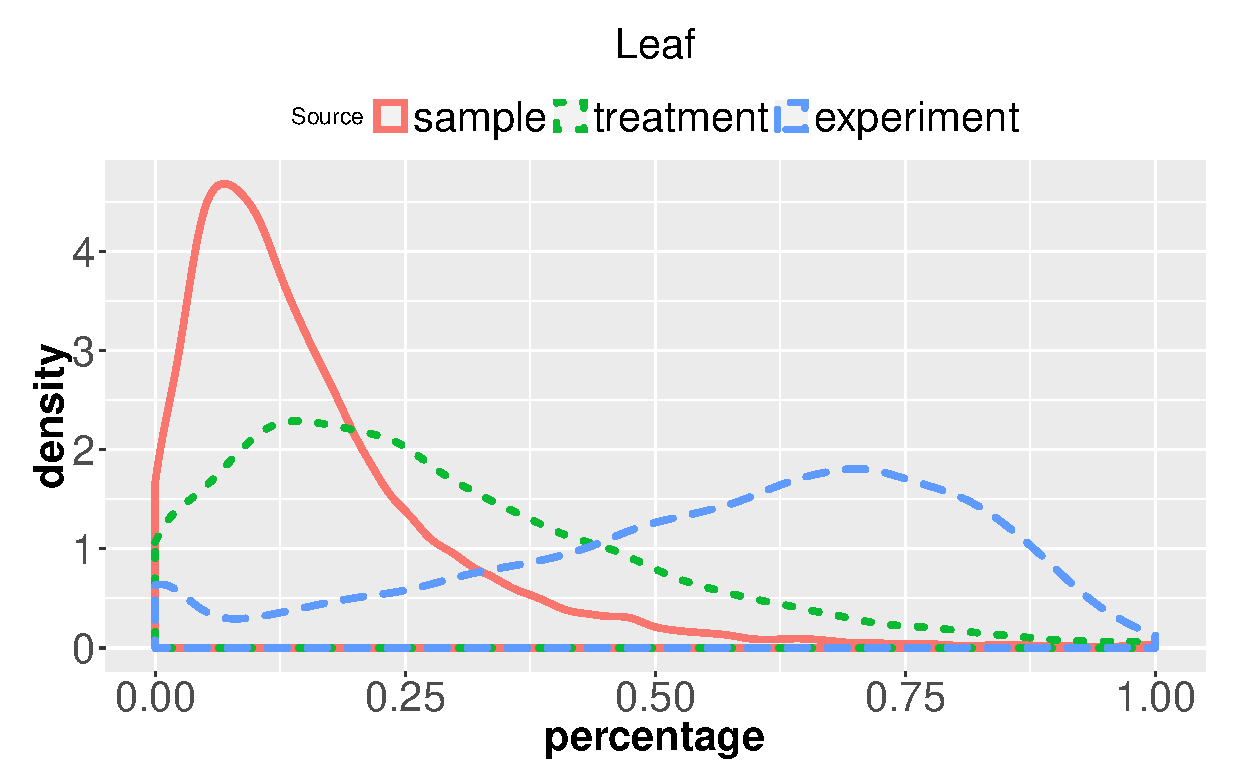
\includegraphics[scale=0.3]{../Figures/var_dens2.eps}
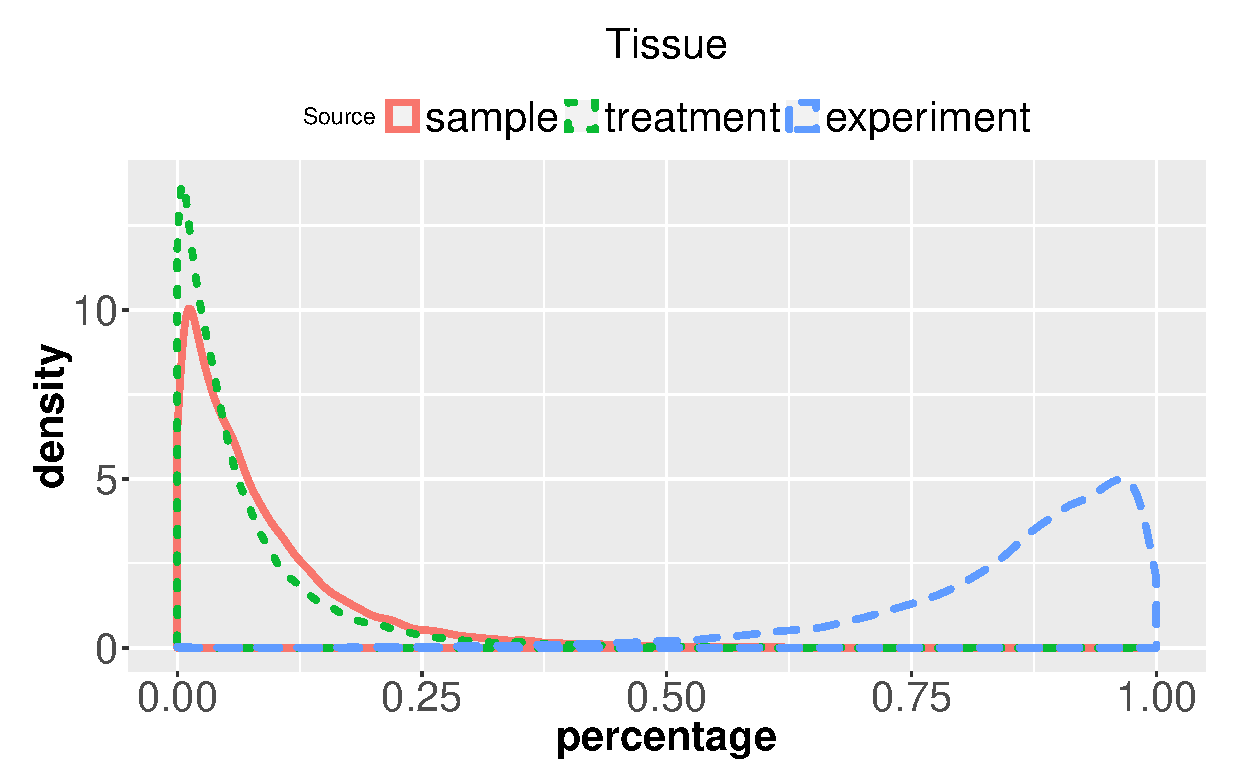
\includegraphics[scale=0.3]{../Figures/var_dens3.eps}
\caption{\label{densityplot} Density plot of variance component: Set 1, Set 2, Set 3 (left to right).}
\end{center}
\end{figure} 



\subsection{Normalization}
One particular goal of identifying stably expressed genes is for normalization. As a justification, we used stably expressed genes to see how normalization factors vary by choosing different numbers of reference genes.   We chose top 10, 100, 1000, 10000 stably expressed genes as reference, and then calculated normalization factors by DESeq method for each sample in Set 1, Set 2 and Set 3, respectively. Figure \ref{fig:normfactor} shows paired scatter plot of normalization factors, in which high consistency is reached when top 100 or 1000 stably expressed gene are selected. We recommend to use as reference top 100 or 1000 stably expressed genes  to do normalization.

 \begin{figure}[h!]
\begin{center}
\includegraphics[scale=0.3]{../Figures/norm1_u.eps}
\includegraphics[scale=0.3]{../Figures/norm2_u.eps}
\includegraphics[scale=0.3]{../Figures/norm3_u.eps}
\caption{\label{fig:normfactor} matrix plot of normalization factors by choosing top 10, 100, 1000, 10000 stably expressed genes for Set 1 (A), Set 2 (B), and Set 3 (C). }
\end{center}
\end{figure}

 \begin{figure}[h!]
\begin{center}
\includegraphics[scale=0.5]{../Figures/r3.eps}
\caption{\label{fig:scaled_diss} normalization factors of seedling data with stable genes from tissue }
\end{center}
\end{figure}

  \section{Discussion}
  \textbf{Major findings of the study}
  Normalization is an essential step for accurate inference in RNA-Seq data analysis. Global normalization methods relying on inappropriate reference genes may lead to erroneous conclusions. Therefore it is important to identify a set of reference genes in gene expression analysis.  In this study we identified three sets of stably expressed genes for different organs and tissues of Arabidopsis. We confirmed  that traditional HKGs are not necessarily stable under not only microarray, but also RNA-Seq experiment. Unless properly validated, HKGs  should not be used as reference genes. While \cite{czechowski2005genome} identified novel reference genes for different experimental conditions, we demonstrated that they are not among the best candidates for RNA-Seq study.  Instead, we provide reference genes specifically for RNA-Seq study.   [\textit{Those stably expressed genes should be robust against factors including lab, treatment and sample since they are included as random effects in the regression analysis.  }]
   
   We find that variation in Arabidopsis RNA-Seq experiment is dominated by lab effects. In this paper, random effects model allows us to quantify  between-lab, between-treatment and between-sample variance components for each gene.
On average, between-lab variance can account for 52.8\% to 76.7\% of total variation. The second important source of variation comes from treatment effect (16.2\% - 25.0\%) and biological sample variation is the smallest. 
  \subsection{Data Process}
  A big challenge of this project is to obtain the read counts we needed. Firstly, we have limited read counts directly available in NCBI, and more importantly,  the comparability of existing count data is not validated. Those data were processed differently either in terms of software used, or versions of the same software. Both types of difference would likely introduce bias to the read counts. To avoid these concerns and to collect more data, we decided to process raw fastq file with a unified pipeline. Secondly, converting fastq format (up to 10 gigabytes per sample)  into read-count format is computationally intensive, making it essential to select adequate aligner. Two aligners were tested and compared: the standard pipeline in \cite{anders2013count} andSubread in \cite{liao2013subread}.  Our experiment shows that:  in terms of accuracy, the two procedures are comparable to each other; however, in terms of efficiency, the latter is at least three times as fast as the former. As a result, we used Rsubread to process all samples in this paper.

To assure comparability between data sets, we pre-screened experiments by several conditions. First, we only targeted on those lab experiments that have biological replicates for each treatment. Second, we selected experiments whose library layout were single-end. Third, we randomly chose one time period if there were repeated measurements over time, or one run if there were multiple runs. Fourth, we chose experiments with DESeq normalization factors ranging from 0.75-1.25 after we had all the read counts. We investigated all the Arabidopsis experiments available at NCBI up to August 31, 2014.

  \subsection{Alternative method}
Another widely adopted approach of fitting GLMM to the data is via negative binomial (NB) regression. In many cases,  RNA-Seq data analysis begins with the assumption that $Y_{jkl}$ follows a negative binomial distribution (a.k.a Poisson-Gamma mixture) which introduces a dispersion parameter to capture the extra-Poisson variation.  In the negative binomial regression, we tried to estimate between experiment and between treatment variation. Specifically,  for each gene, we assume $Y_{jkl}\sim NB(\mu_{jkl}, \phi)$ with the link function
 \[\log(\mu_{jkl})= \xi + \log(R_{jkl}N_{jkl}) + \alpha_l + \beta_{k(l)}\]
where similarly, $\alpha_l$ is the random effect for experiment, and $\beta_{k(l)}$ is random treatment effect nested in experiments.  The only difference is that the dispersion $\phi$, rather than variance of biological sample in Poisson regression, is estimated in NB setting. We saw no significant difference in estimating the variance components between these two approaches. The NB regression is done by \verb"glmer.nb()" in \verb"lme4" package\citep{bates2012lme4} and \verb"glmmadmb()" in \verb"glmmADMB" package\citep{bolker2012getting}. Unfortunately, both implementations of NB regression experienced convergence failure. \\

A limitation of this study is that the inherent design structures are not taken into account unless when the experiment is a case-control (single factor) study. Our concern is two fold: one, although we collected more than 150 samples, they are far from enough for a complicated design structure because usually there are only 2 or 3 replicates within each treatment;  two, efficient algorithm is not available for generalized linear mixed model with more than three random effects \citep{bolker2009generalized}. 

\section{Supplementary Material}
The details of experimental data is summarized as below

\subsection{Set 1}
\begin{landscape}
\begin{table}
\footnotesize
\centering
\begin{tabular}{p{2cm}p{2cm}p{1cm}p{4cm}p{2.4cm}p{3cm}p{4cm}} \hline
GEO Number &Tissue cluster & sample Size & Description & Age  &Col Name & Platform\\ \hline
GSE37159 &seedling &8	& Col-0, bzr1-1D, pifq and pifq;bzr1-1D  grown on BRZ-containing medium in the dark & 5 days &GSM912634-GSM912641 & Illumina HiSeq 2000\\  \hdashline
GSE38879 &seedling &12 & Transgenic line rve8-1 RVE8::RVE8:GR and rve8-1 treated with DEX or mock with three biological replicates each, 12 samples in total & 7 days  &GSM951349-GSM951360  &Illumina HiSeq 2000\\ \hdashline
GSE43865 &seedling & 6  & wild-type and link1link2 mutant plants were grown for two weeks under continuous white light conditions at 22 degrees centigrades & 9 days & GSM1072464-GSM1072469 &Illumina Genome Analyzer IIx  \\	\hdashline
GSE48767 &seedling & 6 &The wild-type seedlings and the phyA-1 mutant were grown, within each 3 biological replicates available & 4 days   &GSM1184353-GSM1184358, GSM1401633-GSM1401638 &Illumina HiSeq 2000 \\ \hdashline
GSE51119 &seedling  & 10  & homozygous ibh1(SALK 049177), ibl1(SALK 119457), 35Spro:IBH1-GFP and 35Spro:IBL1-GFP were compared to wild type (Col) &10 days  & GSM1239079-GSM1239088 &Illumina HiSeq 2000 \\ \hdashline
GSE51772 &seedling  & 8  & Col-0 and iaa3 were grown on medium for 5 days and treated with mock or 100 nMBL for 4 hr &5 days  & GSM1252262-GSM1252269 &Illumina HiSeq 2000 \\ \hdashline
GSE53078 &seedling &4 & Compare the transcriptome of HBI1-Ox and wild type & 5 days &   GSM1281703-GSM1281706 &Illumina Genome Analyzer \\ \hdashline
GSE57086 &seedling & 6  & cR-grown WT and hid1, three biological replicates for each group & 5 days &GSM1390693-GSM1390698 &GPL13222 \\ \hdashline
GSE58082 &seedling &6  &GFP-FHY1 fhy1-1 transgenic,  fhy1-1 mutant  were grown under the same light conditions used (D4d+FR3h)& 4 days &GSM1400495-GSM1400500 & GPL13222 \\ \hdashline
\end{tabular} 
\end{table}
\end{landscape}


\begin{landscape}
\subsection{Set 2}
\begin{table}
\footnotesize
\centering
\begin{tabular}{p{2cm}p{3cm}p{1cm}p{4cm}p{2.4cm}p{3cm}p{4cm}} \hline
GEO Number &Tissue cluster & sample Size & Description & Age  &Col Name & Platform\\ \hline
 GSE35288 &flower &6  & 3 biological replicates of Col-0 wild type and 3 biological replicates of the hae-3 hsl2-3 double mutant &  stage 15  &SRR401413-SRR401430 &Illumina HiSeq 2000 \\ \hdashline
GSE35408 &Hypocotyl & 10 &bzr1-1D and WT were grown in media containing 1uM PAC and 0 or 2uM PPZ for 4.5 days in dark, then treated with 10uM GA3 or mock solution for 12 hr & 4.5 days  & GSM867674-GSM867678, GSM951964-GSM951968  & Illumina HiSeq 2000 \\ \hdashline
GSE48235 &rosette leaves & 6  & For each condition (water, S1, and S3) the transcriptome was sequenced for two replicates & 9 days & GSM1072464-GSM1072469  &Illumina Genome Analyzer II \\	\hdashline
GSE53952 &seed   & 9 	& Three lines of Arabidopsis, fae1/CL37/PDAT were generated & 7-12 days & GSM1303953-GSM1303979 &Illumina Genome Analyzer IIx etc.. \\  \hdashline
GSE56326 &carpels (15 developing inflorescences) & 8 &Expression profile comparation of wild type, nga mutant and NGA overex- pression &stage 8-13&  & 	Illumina HiSeq 2000 \\ \hdashline
\end{tabular} 
\end{table}
\end{landscape}
\begin{landscape}
\subsection{Set 3}
\begin{table}
\footnotesize
\centering
\begin{tabular}{p{2cm}p{3cm}p{1cm}p{4cm}p{2.4cm}p{3cm}p{4cm}} \hline
GEO Number &Tissue cluster & sample Size & Description & Age  &Col Name & Platform\\ \hline
GSE36626 &leaves & 4 &Analysis of 2 different histone H3 variants and transcriptome in 2 conditions.  & 4 weeks &GSM897684-GSM897687 & Illumina Genome Analyzer IIx \\ \hdashline
GSE39463 &leaves  &12		&Columbia-0 pen2-1 pad4-1 sag101-2 mutant, and samples were collected at 24 hours post inoculation (hpi) of Bgh & & &Illumina HiSeq 2000 \\ \hdashline
GSE48235 &leaves & 6  & For each condition (water, S1, and S3) the transcriptome was sequenced for two replicates & 9 days & GSM1072464-GSM1072469  &Illumina Genome Analyzer II \\	\hdashline
GSE51304 &leaves  & 18 &Bisulfite-seq data for cmt2-7 single mutants, cmt3 single mutants, drm1/2 double mutants, drm1/2 cmt3 triple mutants are collected  & 3 weeks & GSM1242374-GSM1242391 &GPL13222 \\ \hdashline
GSE54677 & leaves   &20  &Col morc1 morc2 morc6 and their double mutants. For each sample, two biological replicates were performed &adult & GSM1321694-GSM1321713	 &	GPL13222\\ \hdashline
\end{tabular} 
\end{table}
\end{landscape}


 \begin{figure}[H]
\begin{center}
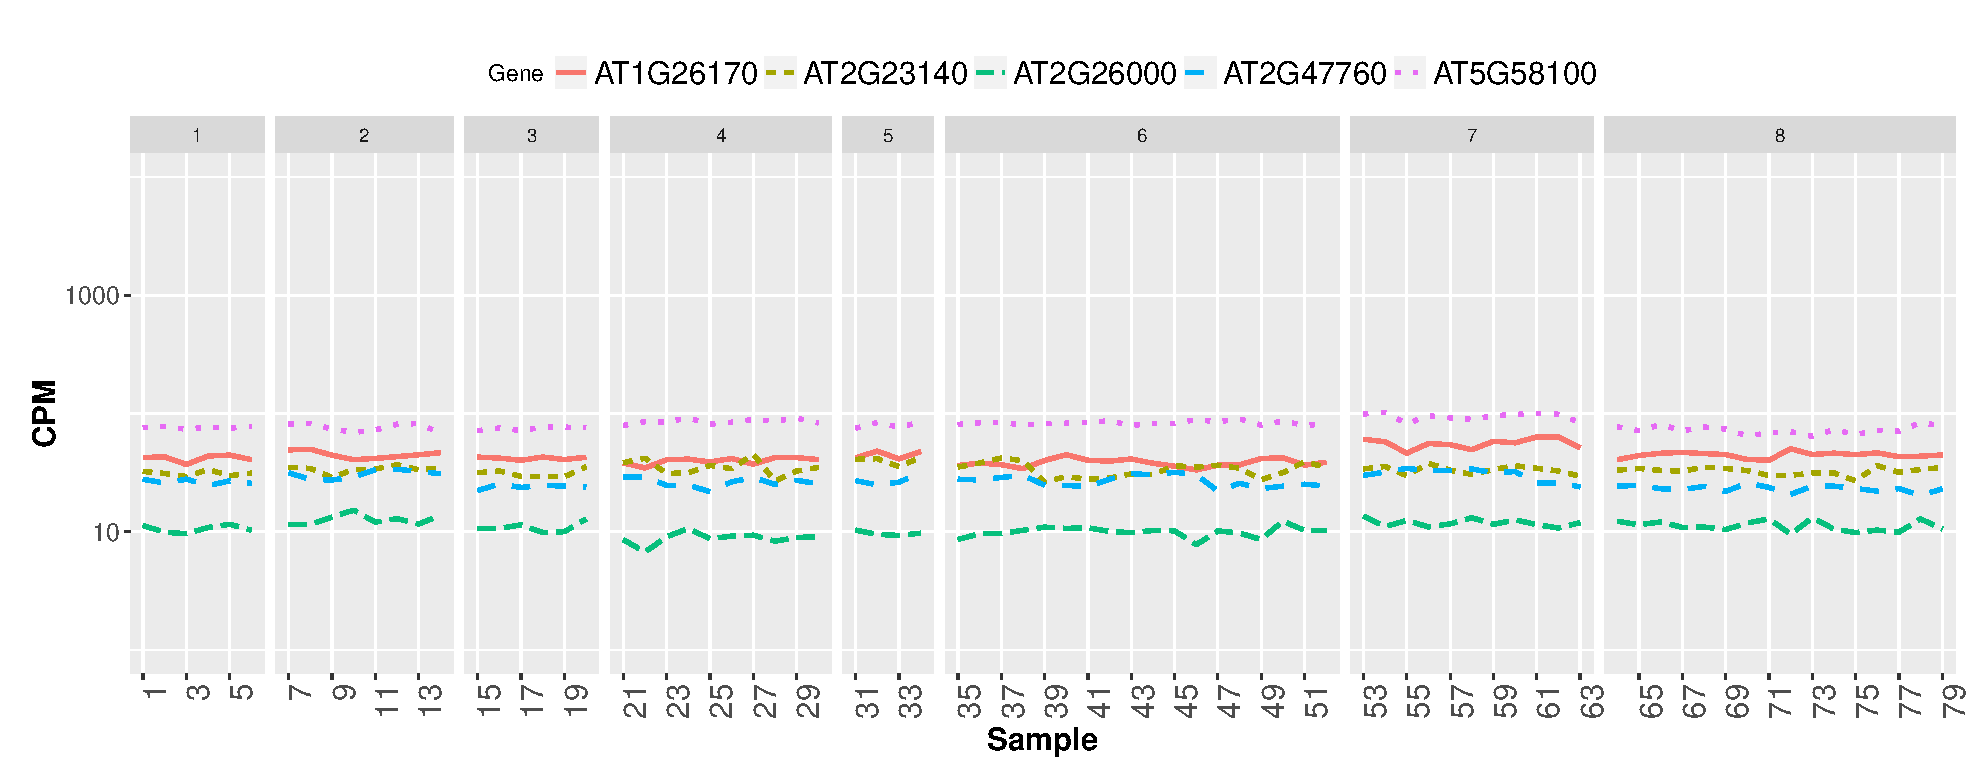
\includegraphics[scale=0.4]{../Figures/A3.eps}
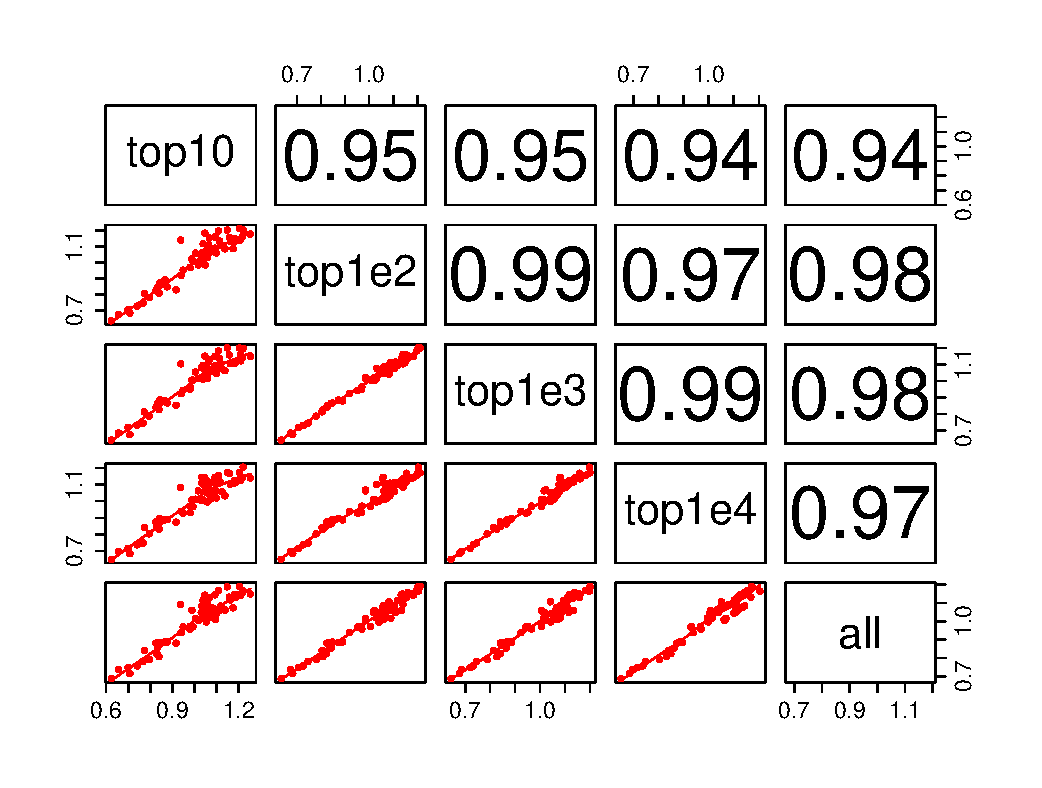
\includegraphics[scale=0.4]{../Figures/B3.eps}
\includegraphics[scale=0.4]{../Figures/C3.eps}
\caption{{\small{\label{sup:expressinlevel} expression levels of Arabidopsis RNA-Seq leaf data: traditional reference genes in set 3 (top)};  5 stably expressed genes by  Czechowski et. al. (middle); 5 stably expressed genes identified by total variance (bottom)}}
\end{center}
\end{figure} 


% \begin{figure}[h!]
%\begin{center}
%\includegraphics[scale=0.5]{../Figures/rank_sl.eps}
%\includegraphics[scale=0.5]{../Figures/rank_st.eps}
%\caption{\label{fig:rankAgainstrank} Rank plot of stably expressed genes,  Set 1 versus Set 2 and Set 3.}
%\end{center}
%\end{figure}

 \begin{figure}[h!]
\begin{center}
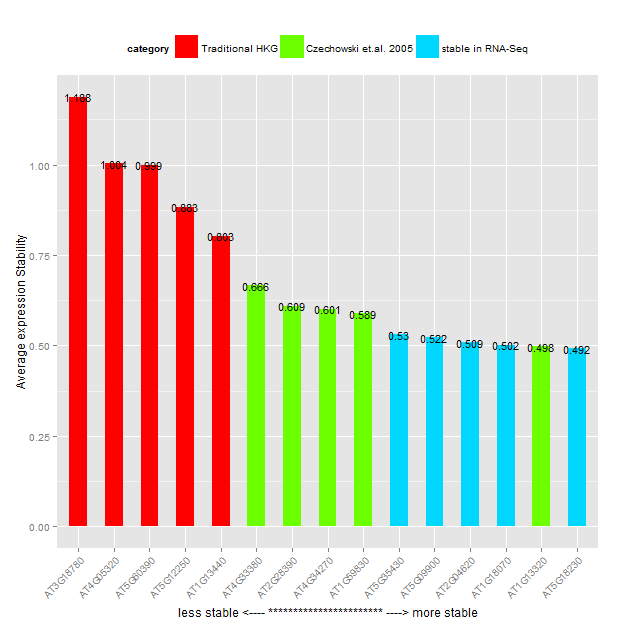
\includegraphics[scale=0.3]{../Figures/mvalue2.png}
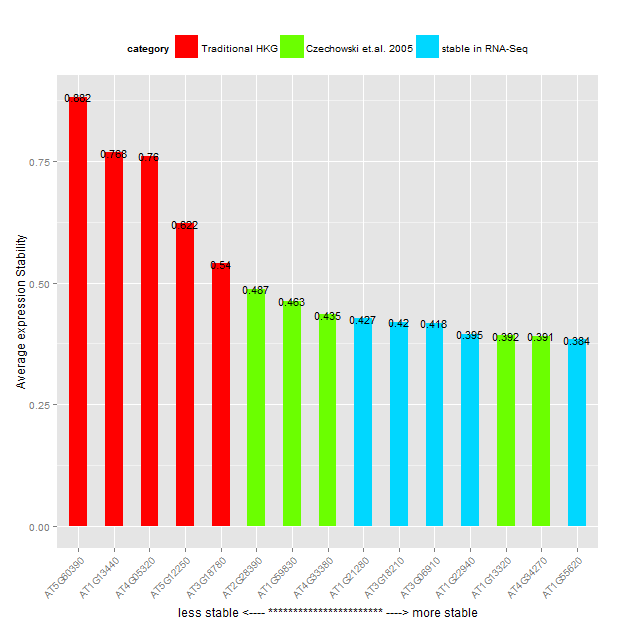
\includegraphics[scale=0.3]{../Figures/mvalue3.png}
\caption{\label{sup:mvalue} geNORM ranking of reference genes: 5 traditional HKGs, 5 reference genes identified by Czechowski et. al. and 8 stably expressed genes based on seedling RNA-Seq data.  The spearman correlations of $M$ values and total variance  are 0.989 and 0.977, respectively. }
\end{center}
\end{figure}


\newpage


\bibliographystyle{apalike}
\bibliography{mybib}

\end{document}

